\documentclass[../Main/main.tex]{subfiles}

\begin{document}
\graphicspath{{../numerical results/figs/}}
		\chapter{Numerical results}
		\section*{convergence for homogenous elliptic model problem}
		The convergence tests in this section are similar to some of the tests done in chapter three of \cite{https://doi.org/10.1002/num.20320}. We consider the elliptic model problem.
		\begin{equation} \label{eq:model}
			\begin{split}
				\nabla \cdot \pmb{q} &= f \\
				\pmb{q} &= -\pmb{K}\nabla u
			\end{split}
		\end{equation}
		We set the solution
		\begin{equation}\label{eq:pressure_solution_model}
			u = cosh(\pi x)cos(\pi y)
		\end{equation} 
		And set $\pmb{K}$ to be the identity matrix. We call $u: \mathbb{R}^2 \rightarrow \mathbb{R}$ for the potential and $\pmb{q}:\mathbb{R}^2 \rightarrow \mathbb{R}^2$ for the flux. And both values are of importance wehen solving \eqref{eq:model}. The flux term, $\pmb{q}$, could for example be use to compute the transport of some contaminant in a porous medium.\\
		As in \cite{https://doi.org/10.1002/num.20320} page 1340 we define the normalized discrete $L_2$ norms:
		\begin{equation}
			\left \| u - u_h \right \| =  \left (  \frac{1}{V}\sum_i V_i(u_{h,i}-u_i)^2\right )^{\frac{1}{2}}
		\end{equation}
		\begin{equation}\label{eq:normal_flow_density}
			\left \| q - q_h \right \| =  \left (  \frac{1}{Q}\sum_a Q_a(q_{h,a}-q_a)^2\right )^{\frac{1}{2}}
		\end{equation}
		Where $q_a = -\pmb{\hat{n}} \cdot \pmb{q}$ is the normal flow density over edge $a$, with $\pmb{\hat{n}}$ beieng unit normal to the edge. $q_{h,a}$ is the discrete flux over $a$, $u_{h,i}$ is the discrete potential at cell $i$, and $u_i$ is the potential evaluated at the cell-center. $Q_a$ is the volume associated with edge $a$, ie. the sum of the two volumes sharing edge $a$. $V = \sum_{i} V_i$ and $Q = \sum_{a} Q_a$.
		\par 
		The normal flux density \eqref{eq:normal_flow_density} is easily obtained when working with finite volume methods, it is implicitly computed when assembling the matrix.
		For the finite element method however we use the transmissiblity coefficients from the L-method. As we see in (Cao, Y., Helmig, R. and Wohlmuth, \cite{https://doi.org/10.1002/num.20525}) chapter three, the bi-linear form of the linear lagrange finite element method on triangular grid is equivalent to the flux integral of the L-method for uniform paralellogram grids. When the grid is perturbed as in figure \ref{fig:mesh_perturbed}, this way of computing the normal flow density is not justified and is only approximate. There are other choices of flux recovery from the finite element method. The most obvious one would be to use the piecewise constant gradients on each triangle, with a triangle-centered finite volume method. This would however not be a conservative method, and one would get numerical diffusion when solving the corresponding transport equation.\\
		\begin{figure}
			\label{fig:fem_flux}
			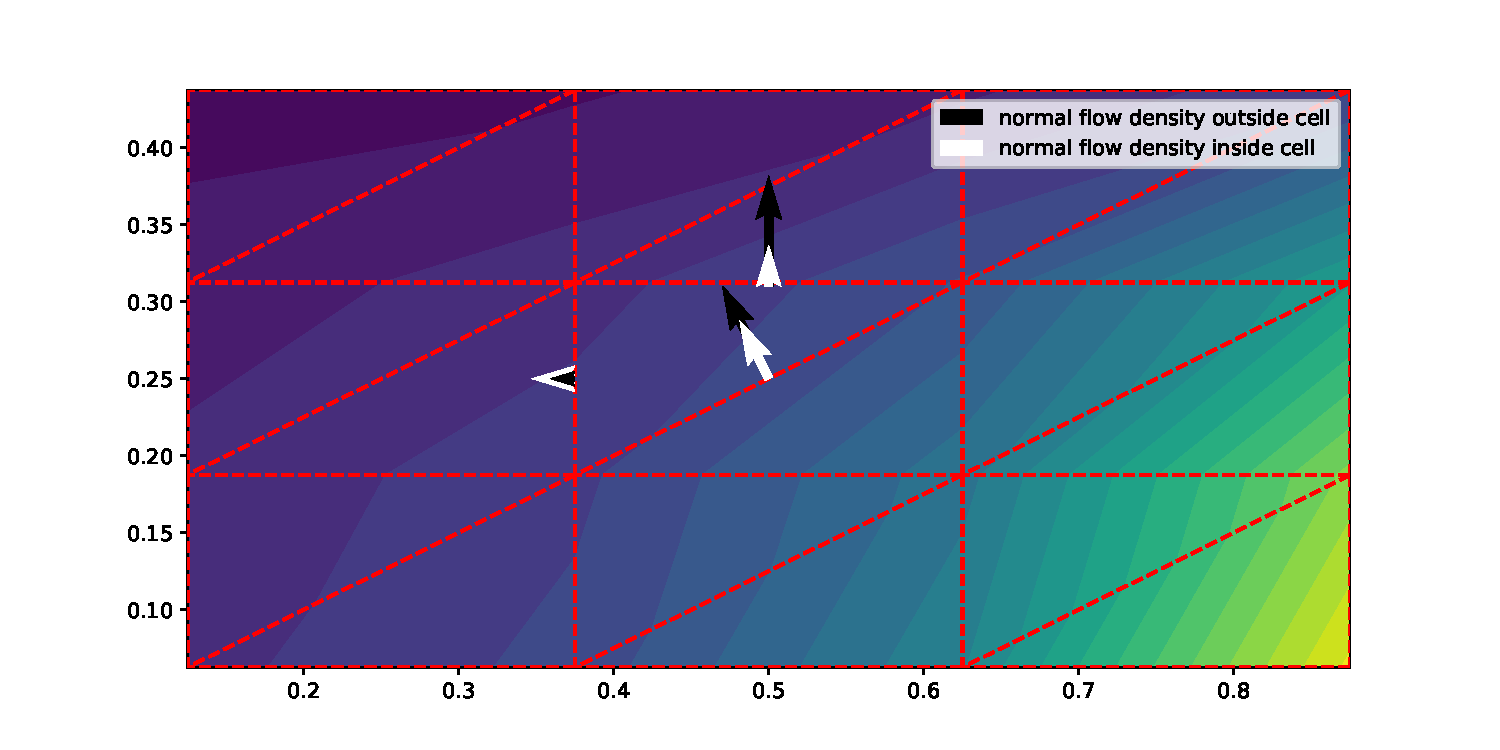
\includegraphics[width=1\textwidth]{fem_flux.pdf}
			\caption{An illustration of why it's a bad idea to use the piecewise constant gradient on each element for computing normal flow. The normal flow is discontinuous across the edges, and flow into the cell is not equal to flow out.}
		\end{figure}
		In the first setup with uniform rectangular mesh, all the methods are identical and we get a quadratic convergence for normal flow density and potential as we see in figures \ref{fig:mesh_uniform_potential} and \ref{fig:mesh_uniform_flow}.\\
		In the second setup with uniform trapezoidal mesh illustrated in figure \ref{fig:mesh_trapezoidal} we get quadratic convergence for normal flow density and potential, except for TPFA. This method is  not convergent for grids that are not K-orthogonal, see figures \ref{fig:mesh_trapezoidal_potential} and \ref{fig:mesh_trapezoidal_flow}.\\
		In the perturbed mesh setup \ref{fig:mesh_perturbed}, the convergence rate for the normal flow density drops to about $O(h)$ in the $L^2$ norm and even worse for the max norm, see figures \ref{fig:mesh_perturbed_potential} and \ref{fig:mesh_perturbed_flow}.\\
		The next setup is with perturbed mesh and an aspect ratio of $0.1$, see figure \ref{fig:mesh_perturbed_1d2} for an illustration of aspect ratio $0.5$. Here we clearly see that the O-method performs worse than the other two. We also see that the finite element method is the only method to achieve quadratic covergence for the potential.
		\begin{figure}[h]
			\centering
			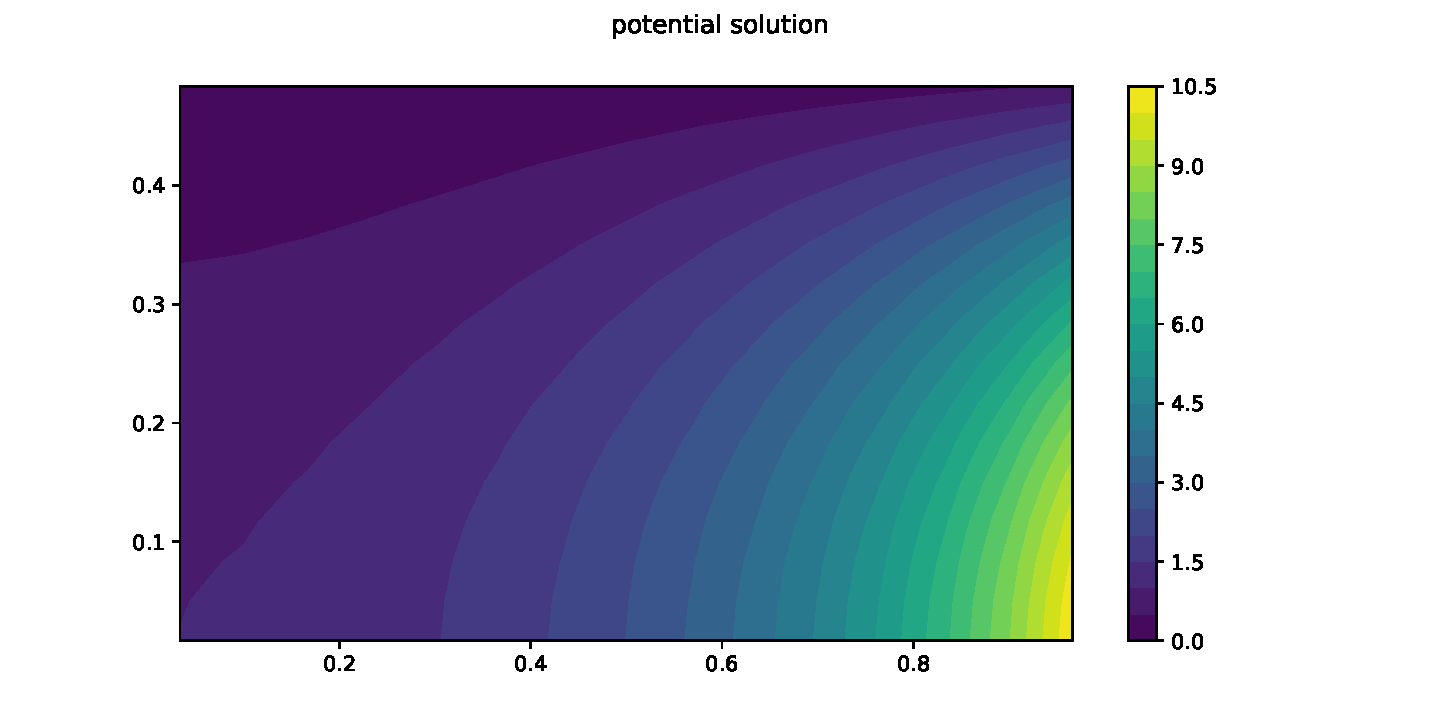
\includegraphics[width=1\textwidth]{Potential.pdf}
			\caption{The solution \eqref{eq:pressure_solution_model} on half the unit square }
			\label{fig:solution}
		\end{figure}
		\newpage
		\begin{figure}[H]
			\centering
			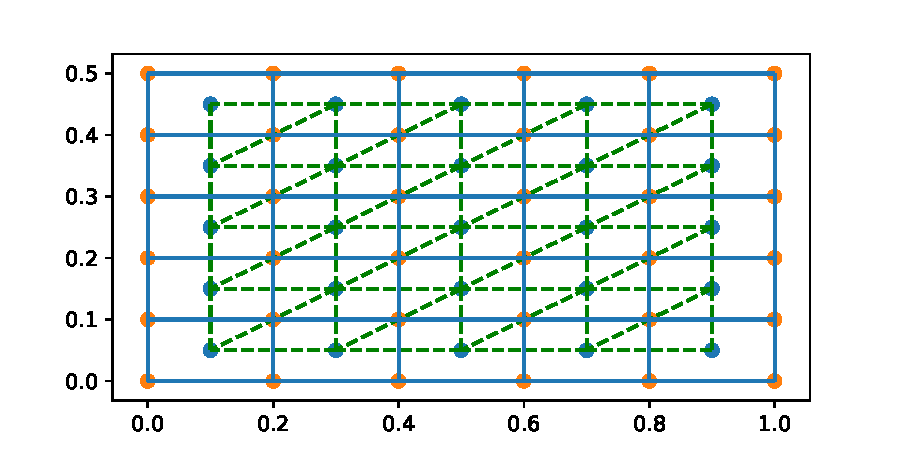
\includegraphics[width=0.8\textwidth]{mesh_quadratic.pdf}
			\caption{Unifrom rectangular mesh on half the unit square. The triangles are used for the finite element solution and are spanned between the nodes of the cell centers of the finite volume methods.}
			\label{fig:mesh_uniform}
		\end{figure}
		\begin{figure}[H]
					\advance\leftskip-1cm
			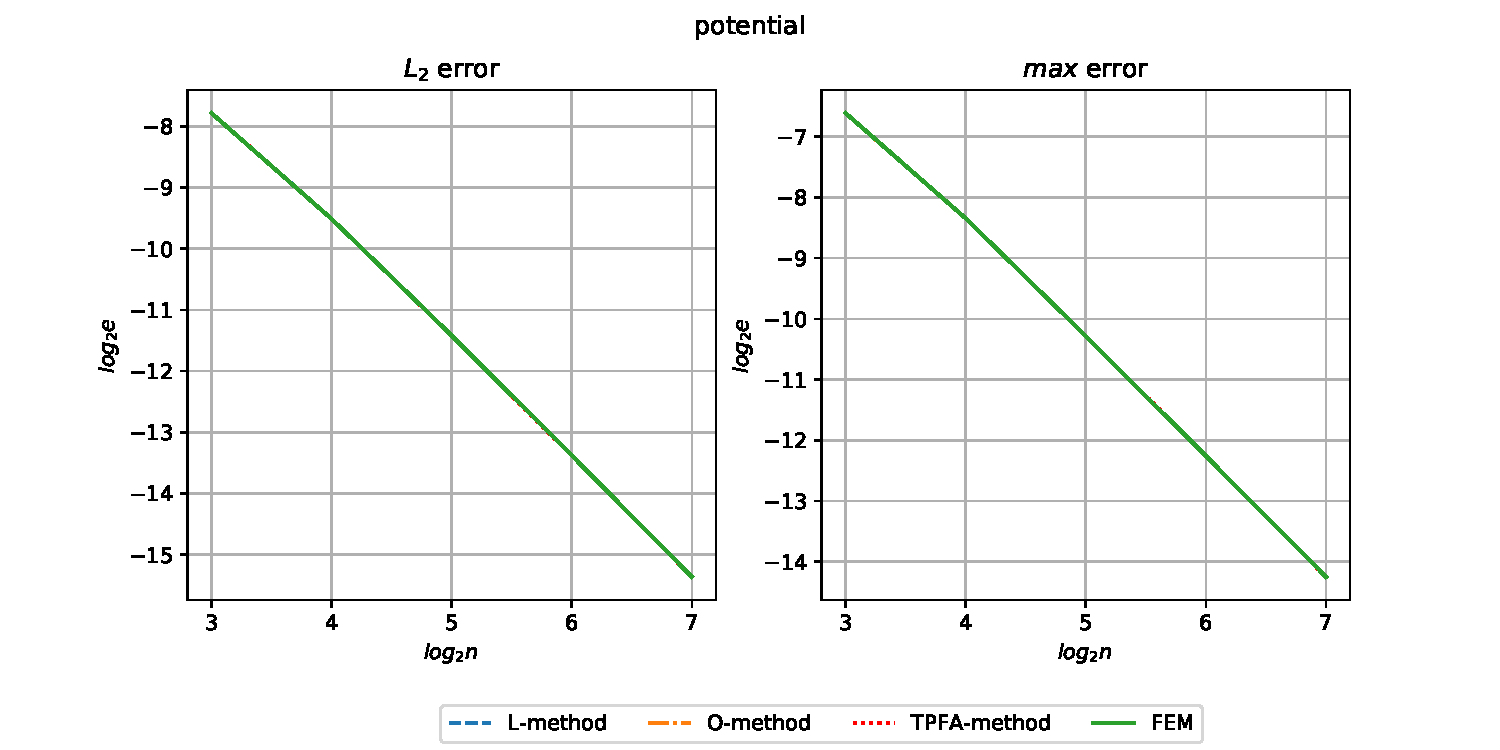
\includegraphics[width=1.2\textwidth]{pressure_quadratic.pdf}
			\caption{Potential error on refinements of the uniform rectangular mesh \ref{fig:mesh_uniform}}
			\label{fig:mesh_uniform_potential}
		\end{figure}
		\begin{figure}[H]
			
			\advance\leftskip-1cm
			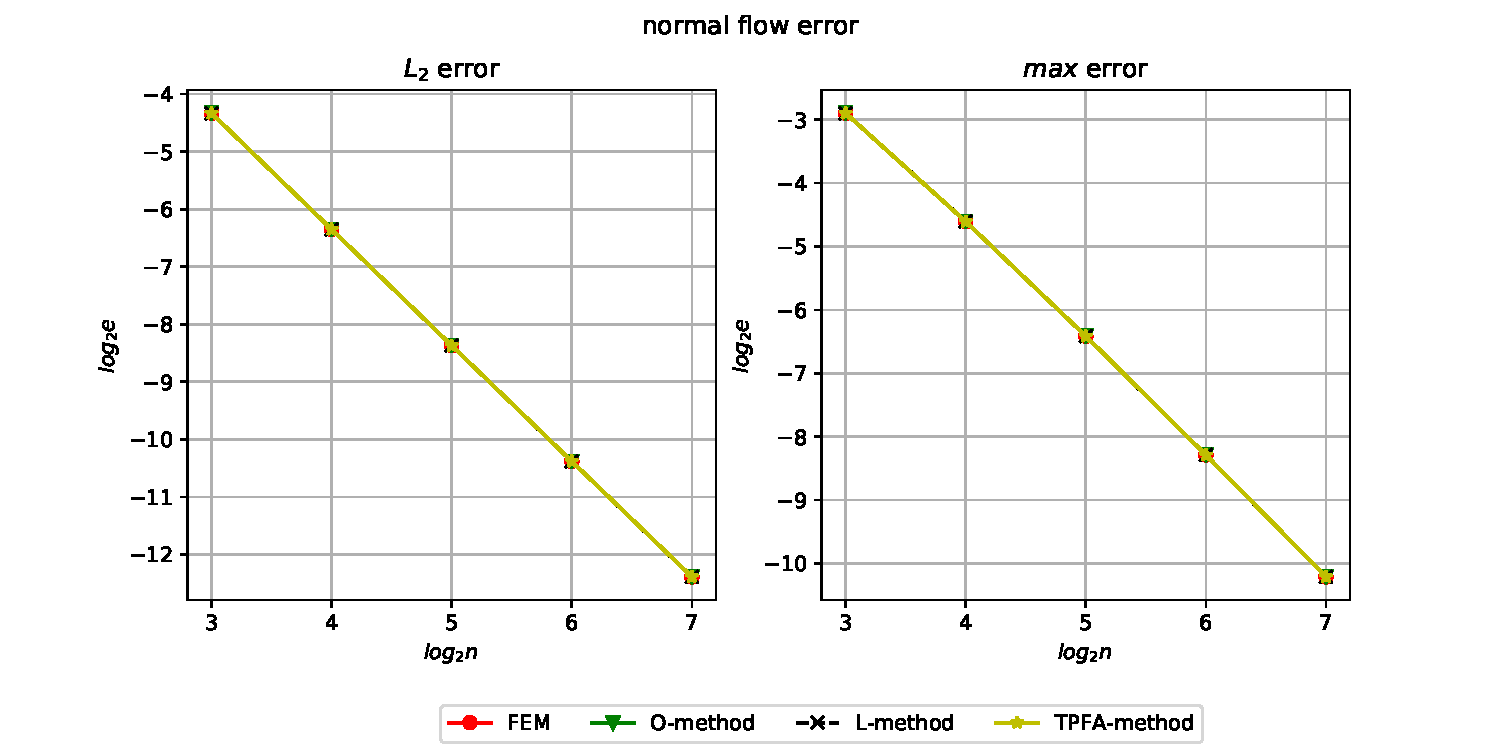
\includegraphics[width=1.2\textwidth]{flow_quadratic.pdf}
			\caption{Normal flow density error on refinements of the uniform rectangular mesh \ref{fig:mesh_uniform}}
			\label{fig:mesh_uniform_flow}
		\end{figure}

		\begin{figure}[H]
			\centering
			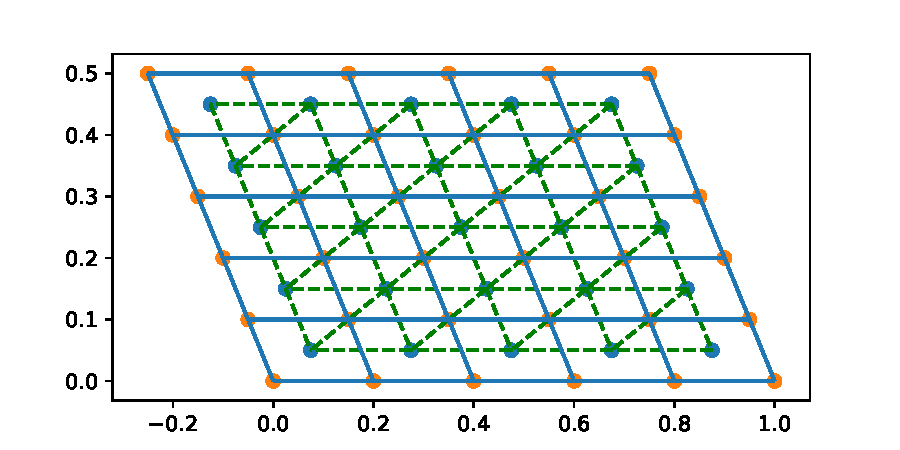
\includegraphics[width=0.9\textwidth]{mesh_trapezoidal.pdf}
			\caption{Trapezoidal mesh, now every point is transformed by $(x,y)  \mapsto (x-0.5y,y)$}
			\label{fig:mesh_trapezoidal}
		\end{figure}
	
	\begin{figure}[H]
		\advance\leftskip-1cm
		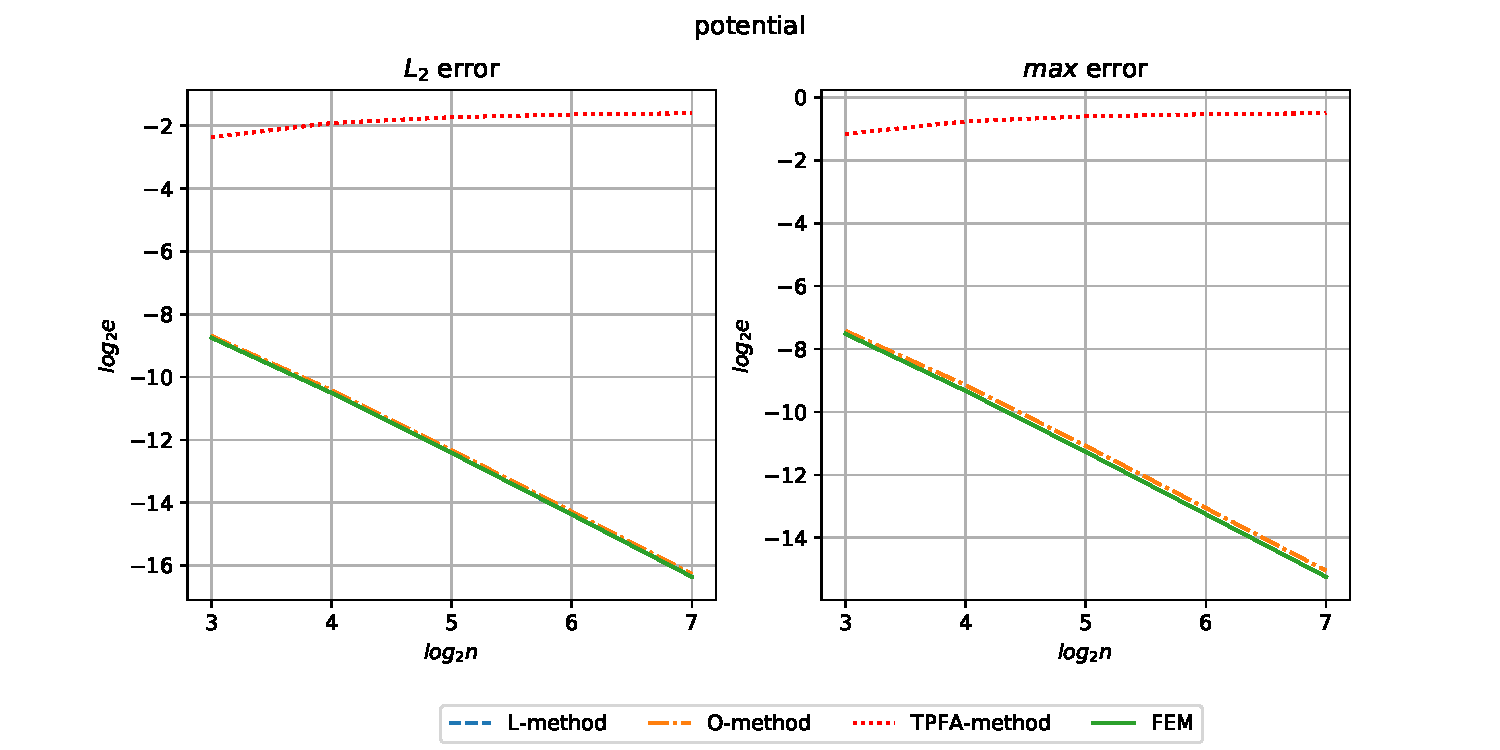
\includegraphics[width=1.2\textwidth]{pressure_trapezoidal_1d1.pdf}
		\caption{Pressure error on refinements of the mesh \ref{fig:mesh_trapezoidal}}
		\label{fig:mesh_trapezoidal_potential}
	\end{figure}
	\begin{figure}[H]
		\advance\leftskip-1cm
		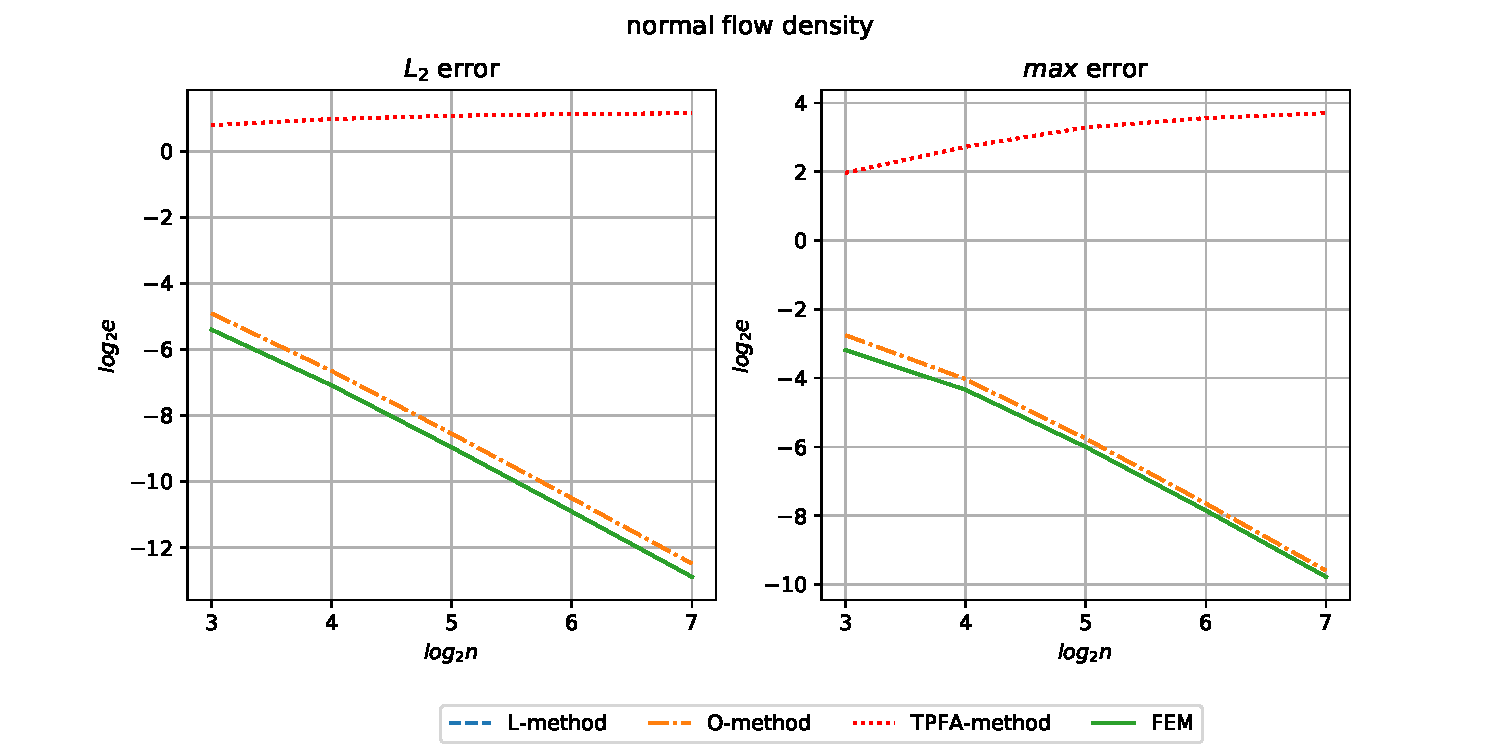
\includegraphics[width=1.2\textwidth]{flow_trapezoidal_1d1.pdf}
		\caption{Normal flow density error on refinements of the mesh \ref{fig:mesh_trapezoidal}}
		\label{fig:mesh_trapezoidal_flow}
	\end{figure}
	
		\begin{figure}[H]
			\centering
			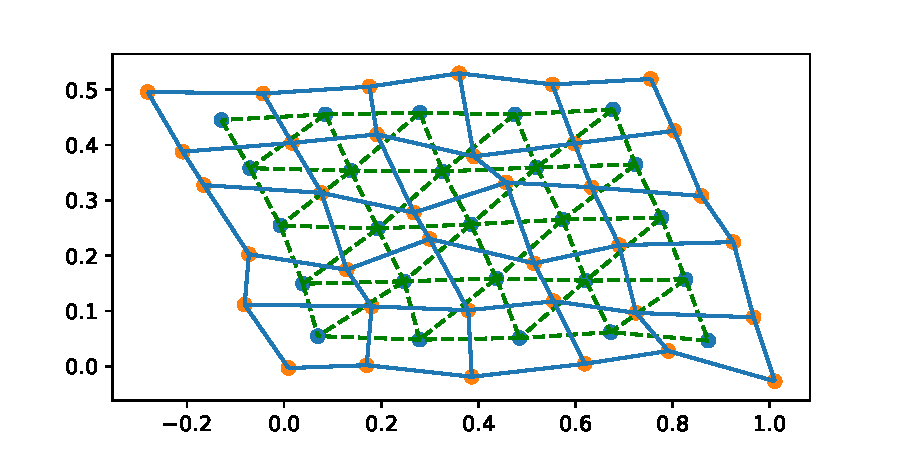
\includegraphics[width=0.9\textwidth]{mesh_perturbed.pdf}
			\caption{Perturbed mesh, every point in the mesh is perturbed by a random number which is $O(\frac{h}{5})$, in both x and y direction.}
			\label{fig:mesh_perturbed}
		\end{figure}
		\begin{figure}[h]
		\advance\leftskip-1cm
			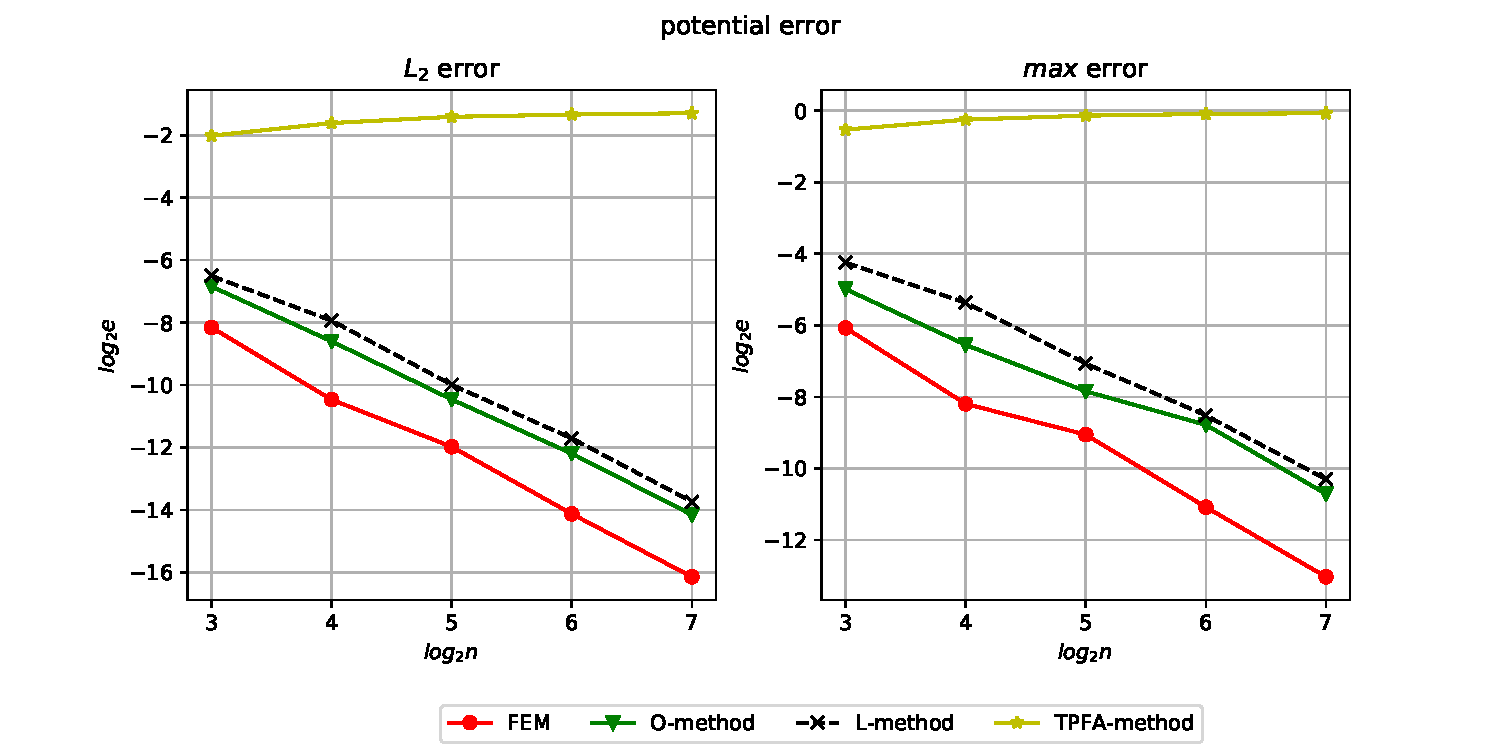
\includegraphics[width=1.2\textwidth]{pressure_perturbed_1d1.pdf}
			\caption{The pressure error of perturbed mesh.}
			\label{fig:mesh_perturbed_potential}
		\end{figure}
		\begin{figure}[h]
		\advance\leftskip-1cm
			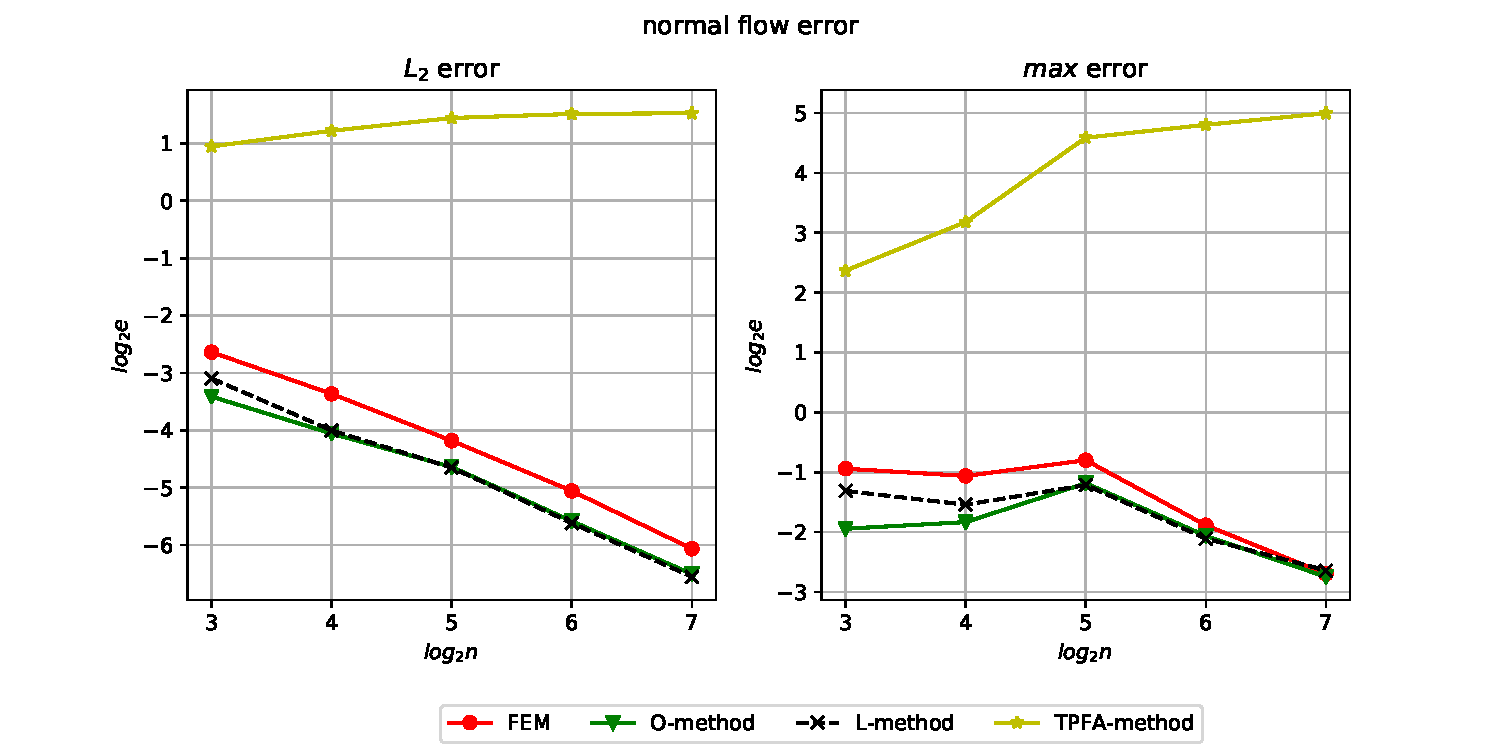
\includegraphics[width=1.2\textwidth]{flow_perturbed_1d1.pdf}
			\caption{The normal flow density error of perturbed mesh}
			\label{fig:mesh_perturbed_flow}
		\end{figure}
		\begin{figure}[H]
			\centering
			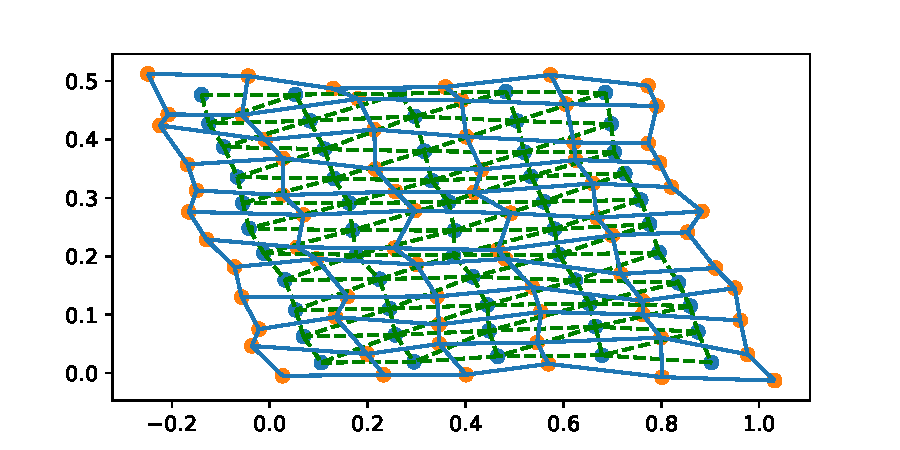
\includegraphics[width=0.9\textwidth]{mesh_perturbed_1d2.pdf}
			\caption{Perturbed mesh with aspect ratio 0.5, there are half as many points in the x-direction as in the y-direction.}
			\label{fig:mesh_perturbed_1d2}
		\end{figure}
		\begin{figure}[h]
		\advance\leftskip-1cm
			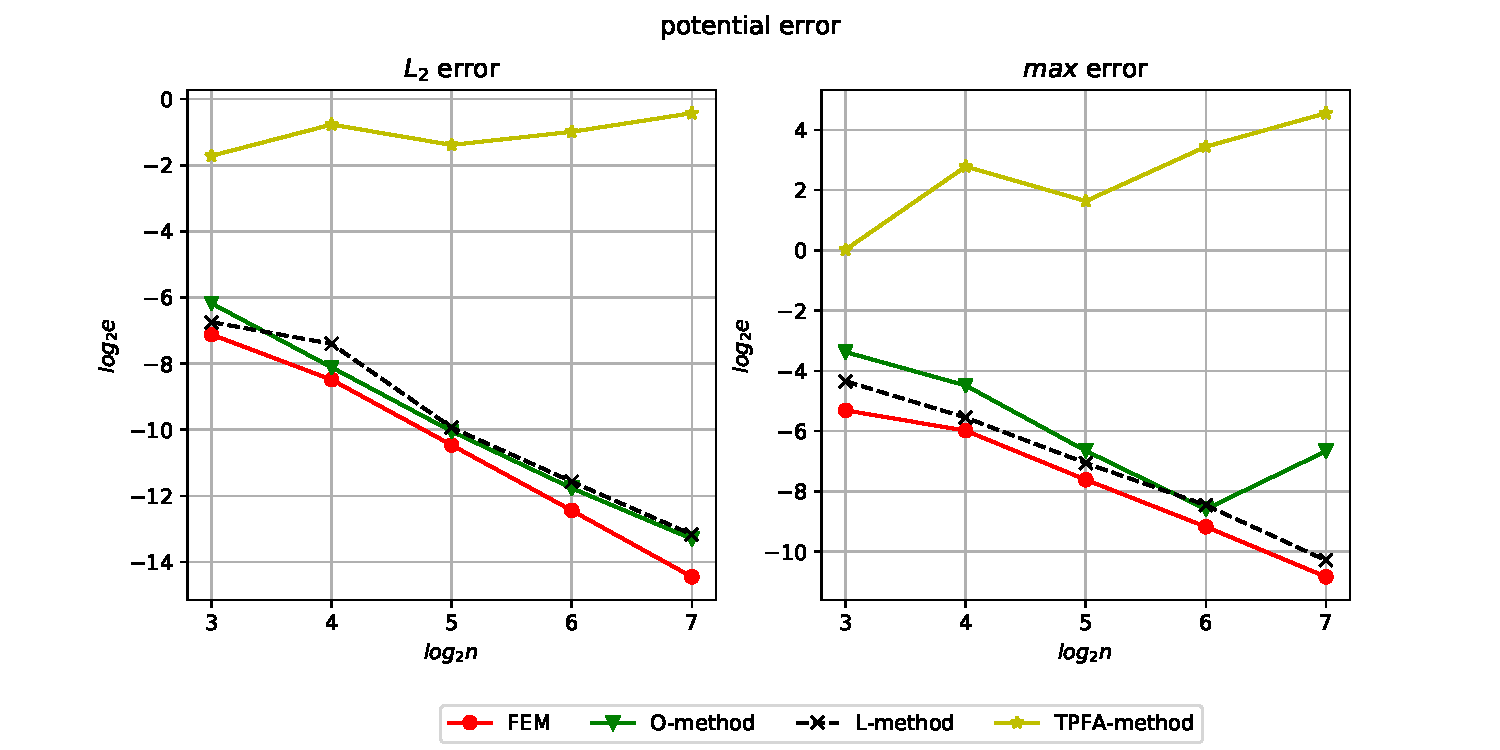
\includegraphics[width=1.2\textwidth]{pressure_perturbed_1d10.pdf}
			\caption{The pressure error of perturbed mesh with aspect ratio 0.1.}
		\end{figure}
			\begin{figure}[h]
			\advance\leftskip-1cm
			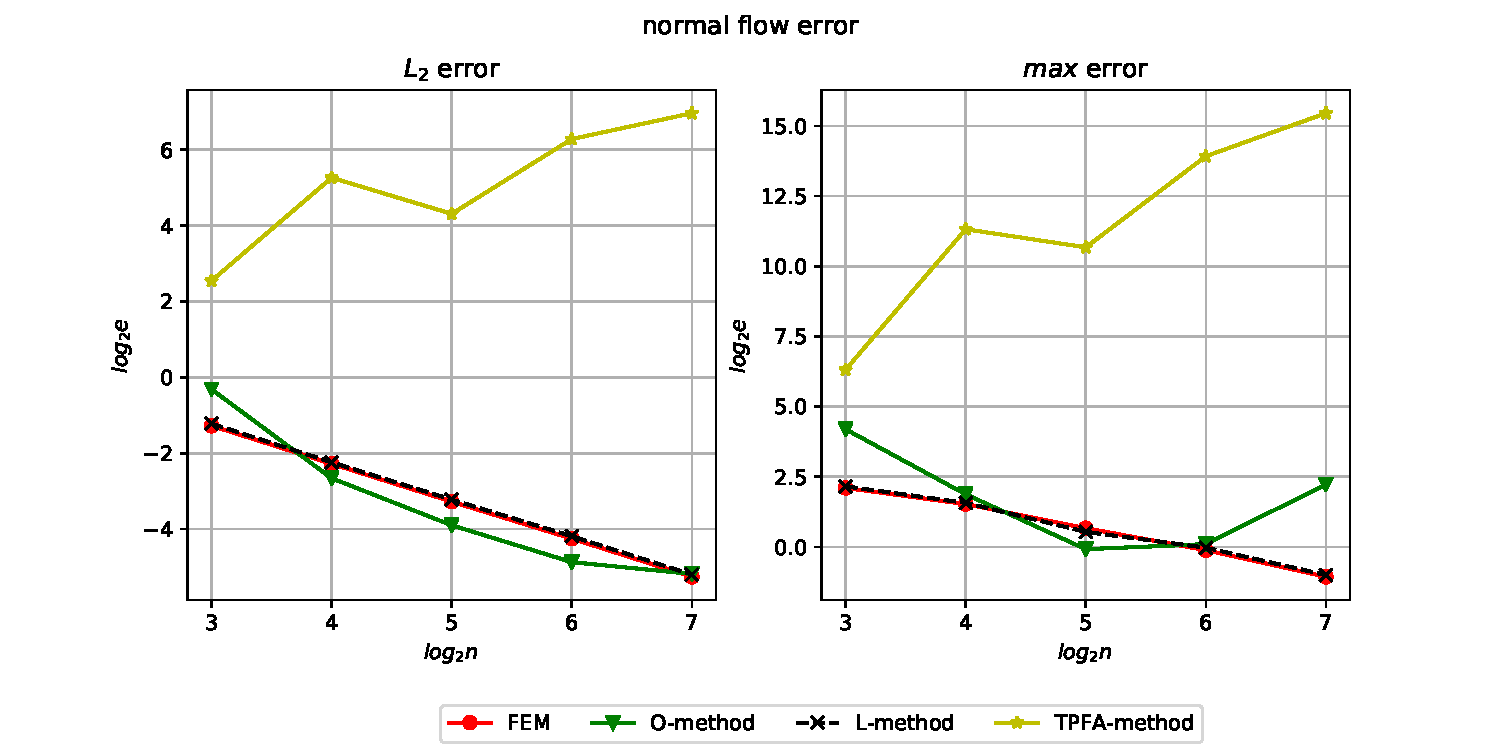
\includegraphics[width=1.2\textwidth]{flow_perturbed_1d10.pdf}
			\caption{The normal flow density error of perturbed mesh with aspect ratio 0.1.}
		\end{figure}
\end{document}